O iodoetano é um líquido incolor usado como precursor em reações orgânicas de alquilação na indústria farmacêutica e na produção de defensivos agrícolas. A decomposição do iodoetano é representada pela equação abaixo. 

\begin{center}
\schemestart
\chemfig{C_2H_5I}(g) \arrow{->} \chemfig{C_2H_4}(g) + \chemfig{HI}(g)
\schemestop
\end{center}

Considere o conjunto de dados apresentado abaixo, obtidos durante o estudo da reação citada:

\begin{center}
\renewcommand{\arraystretch}{1.5}
\begin{tabular}{ c | c c c c}
$k$ & $7,20 \times 10^{-4}$ & $2,20 \times 10^{-3}$ & $1,70 \times 10^{-2}$ & 0,110 \\ 
\hline  
$T$ (K) & 660,0 & 680,0 & 720,0 & 760,0 \\
\end{tabular}
\end{center}

\begin{center}
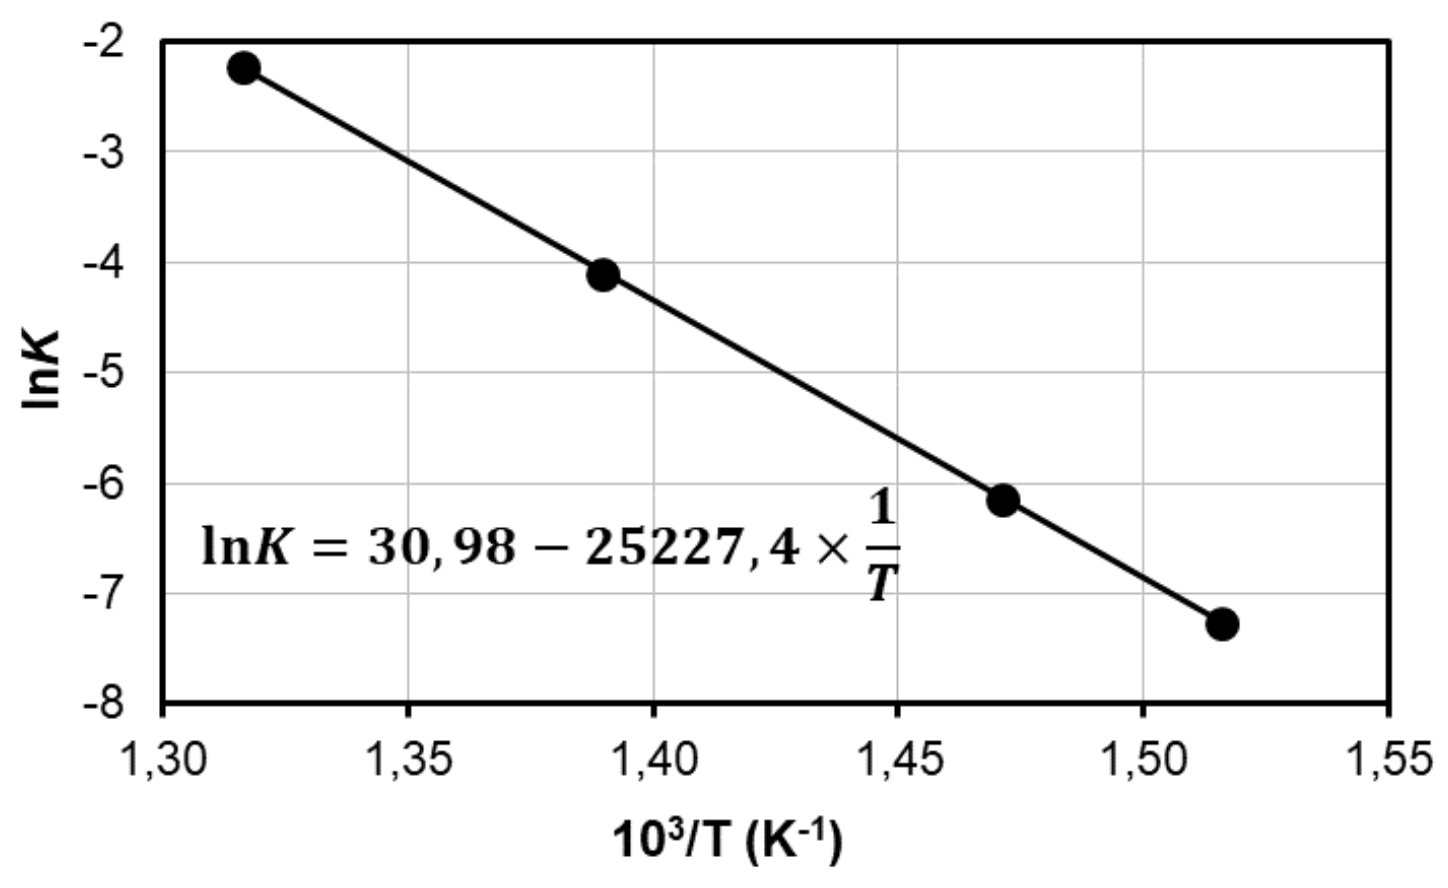
\includegraphics[width=0.5\textwidth]{figure.png}
\end{center}

\begin{enumerate}[label = (\alph*)]
	\item Determine a energia de ativação de Arrhenius para a reação citada e o valor do fator A.
	\item Determine o valor da constante de velocidade da reação à temperatura de 400 $^\circ$C.
	\item Explique como um catalisador influencia na variação de entalpia e constante de equilíbrio de uma reação química. 
	\item Apresente as estruturas de Lewis para o reagente e para os produtos da reaçãp representada, indicado a geometria de cada carbono.
	\item Faça uma previsão comparativa das polaridades do iodoetano, do eteno e do iodeto de hidrogênio.
\end{enumerate}
